\section{Comparison with previous work}

In my study, I investigate the importance of the inner binary's accretion efficiency. The lack of theoretical predictions makes the comparison of the results difficult, but some estimation can be made. The inner binary is expected to accrete more efficiently given the formation of a circumbinary disk instead of a common envelope like -structure \citep{zwart2019triple}. In the case of the former, \cite{zwart2019triple} reports values up to $\beta \gtrsim 0.8$, while in my study the model with the highest accretion efficiency corresponds to $\beta = 0.53$, see \cref{fig:inclination_binary_eff}. Furthermore, for the same model, I find that a value of $\eta \approx 4$ can describe the evolution of the semi-major axis of the outer orbit. Values of $\eta = 3-4$ are reported also by \cite{de2014evolution, zwart2019triple}. Additionally, values of $\eta \gtrsim 3$ are derived in \cite{portegies1995formation} by matching the orbital evolution and birthrate of Be-type X-ray binaries that experience non-conservative mass transfer.

\cite{de2014evolution} simulate the phase of mass transfer for the $\xi$ Tau system using AMUSE. Their study focuses on the effect of the initial mutual inclination on the evolution of the system. They also encounter mass transfer that leads to a common envelope-like structure around the inner binary. Except for the evolution of the inner semi-major axis, the evolution of the outer and inner orbits in my study is qualitatively similar to their results. On the one hand, in \cref{sec:resolution} I demonstrate that the resolution of my simulations is probably poor, hence this may be a reason behind this discrepancy. On the other hand, \cite{de2014evolution} claim to use the same resolution. Their study covers a larger mass transfer duration, $\sim 40$ yr, but this expected as in my case the widening of the inner orbit brings the system relatively fast to the unstable regime. In conclusion, my results qualitatively agree with \cite{de2014evolution} study, but higher resolution simulations are needed to confidently conclude about the evolution of the inner semi-major axis during the mass transfer.

Finally, \cite{zwart2019triple,leigh2020mergers} report that given the formation of a circumbinary disk via RLOF by the outer star, a preferable accretion towards the less massive binary component occurs. Despite the fact that in my simulations no disk forms, I encounter the same behavior for the models wiht $i_{mut} \neq 0^{\circ}$, see \cref{fig:inclination_binary_eff}
\begin{figure}[H]
    \centering
    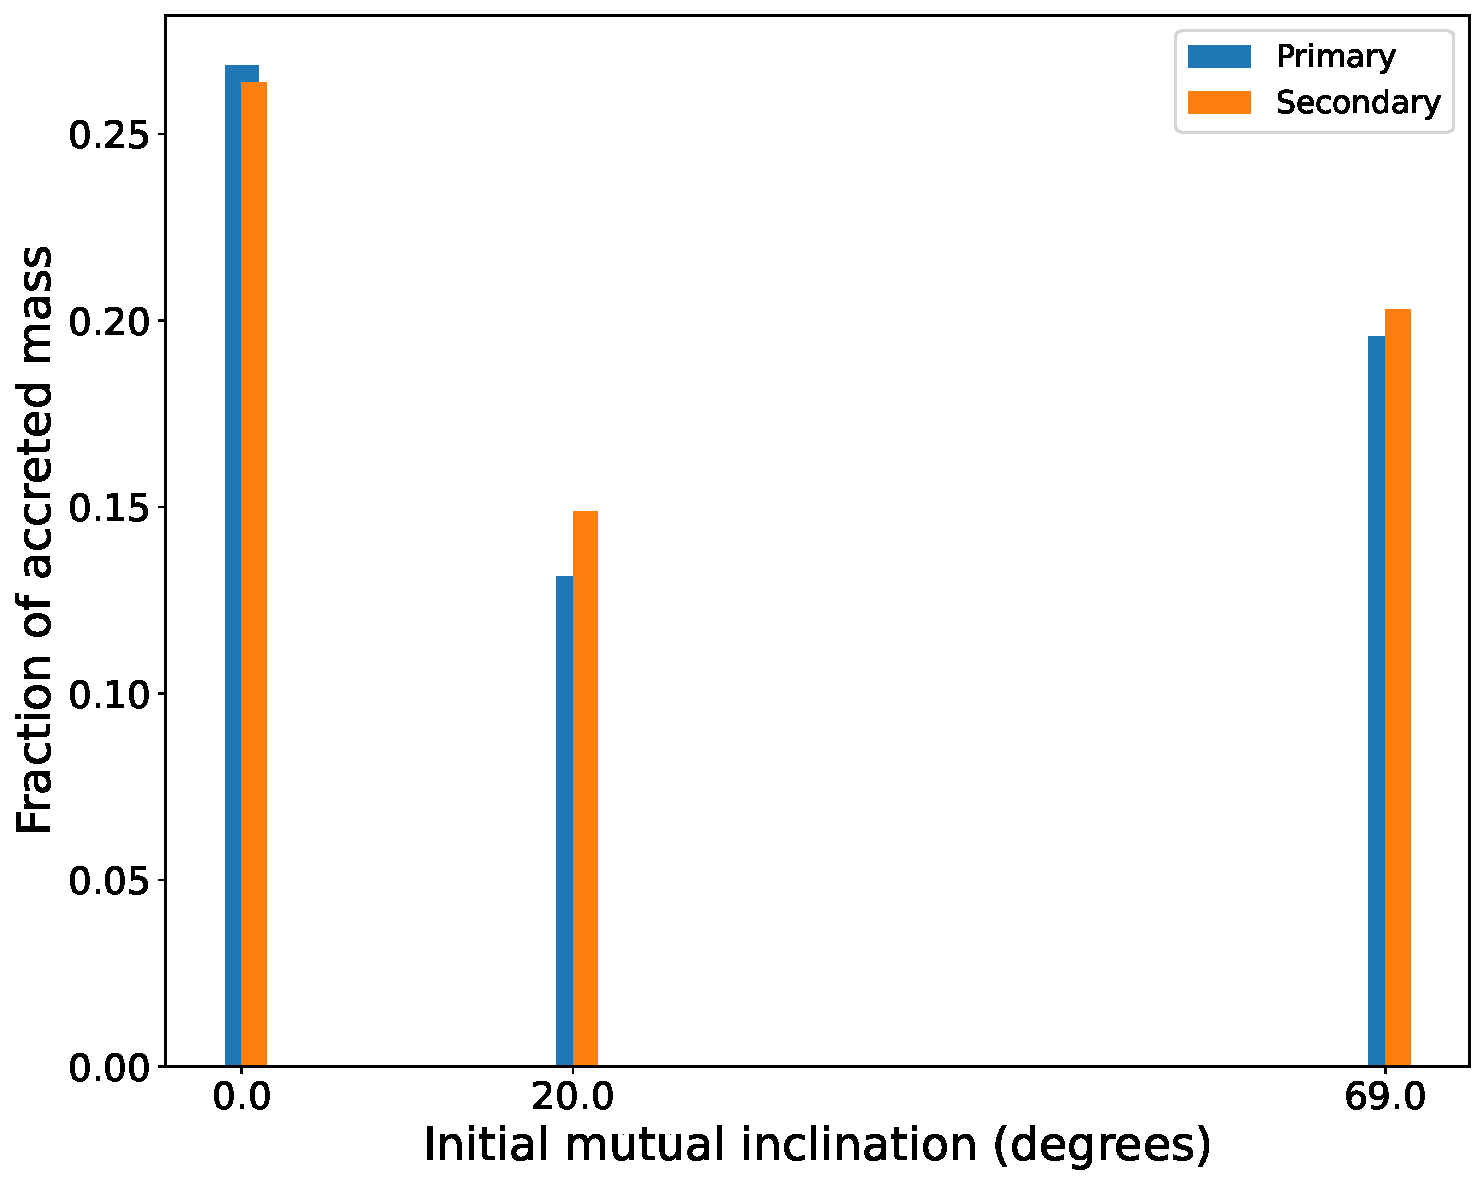
\includegraphics[width=0.9\textwidth]{Thesis/graphs/inclination_case/incliantion_binary_acc_efficiency.pdf}
    \caption{Fraction of the accreted mass by the inner binary stars for different initial inclination of the outer orbit relative to the inner orbit.}
    \label{fig:inclination_binary_eff}
\end{figure}
A solid a description of the aforementioned behavior is not trivial, due to the complicated transport of mass, angular momentum and energy through the accretion stream and throughout the system. More importantly, running higher resolution simulations before trying to interpret this result is necessary. Because gas drag may alter the details of the accretion process. Nonetheless, this outcome is interesting to be investigated due to the fact that it hints towards a mechanism of producing equal mass binaries. 



.